\documentclass{article}
\usepackage{tikz}
\usetikzlibrary{positioning, fit, backgrounds, shapes.geometric, arrows.meta}
\tikzset{
  task/.style={draw, rounded corners=2pt, fill=white, minimum width=26mm, minimum height=8mm, align=center},
  choice/.style={draw, diamond, aspect=2, fill=white, inner sep=1pt, align=center},
  lane/.style={draw=gray!60, fill=gray!8, rounded corners=2pt, inner sep=3mm},
  lane title/.style={font=\bfseries\small},
  group/.style={draw=gray!70, dashed, rounded corners=3pt, inner sep=2mm},
}
\begin{document}
% An expense claim in three swimlanes, one per role, side by side. Each lane
% fits its own steps and the two shared coordinates, so all are as tall.
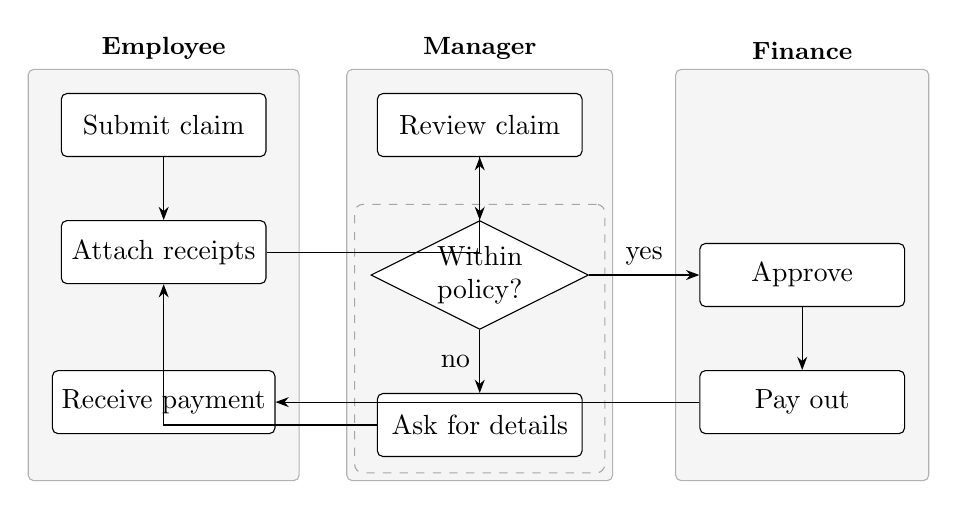
\begin{tikzpicture}[node distance=8mm and 14mm, >=Stealth]
  \node[task] (submit) at (-0.4,0.4) {Submit claim};
  \node[task, below=of submit] (attach) {Attach receipts};
  \node[task, right=of submit] (review) {Review claim};
  \node[choice, below=of review] (within) {Within\\ policy?};
  \node[task, below=of within] (query) {Ask for details};
  \node[task, right=of within] (approve) {Approve};
  \node[task, below=of approve] (pay) {Pay out};
  \node[task] (paid) at (attach |- pay) {Receive payment};

  \draw[->] (submit) -- (attach);
  \draw[->] (attach) -| (review);
  \draw[->] (review) -- (within);
  \draw[->] (within) -- node[auto] {yes} (approve);
  \draw[->] (within) -- node[auto, swap] {no} (query);
  \draw[->] (query) -| (attach.south);
  \draw[->] (approve) -- (pay);
  \draw[->] (pay) -- (paid);

  \begin{scope}[on background layer]
    \coordinate (lanes top) at (submit.north);
    \coordinate (lanes bottom) at (query.south);
    \node[lane, fit=(submit) (attach) (paid) (submit |- lanes top) (submit |- lanes bottom), label={[lane title]north:Employee}] (employee) {};
    \node[lane, fit=(review) (within) (query) (review |- lanes top) (review |- lanes bottom), label={[lane title]north:Manager}] (manager) {};
    \node[lane, fit=(approve) (pay) (approve |- lanes top) (approve |- lanes bottom), label={[lane title]north:Finance}] (finance) {};
    \node[group, fit=(within) (query)] (checks) {};
  \end{scope}
\end{tikzpicture}
\end{document}
